\documentclass[12pt, a4paper, lithuanian]{article}
\usepackage[utf8x]{inputenc}
\def\LTfontencoding{L7x}
\PrerenderUnicode{ąčęėįšųūž}
\usepackage[\LTfontencoding]{fontenc}
\usepackage[lithuanian]{babel}
\usepackage{VUMIFPSkursinis}
\usepackage{cite}
\usepackage{amsmath}
\usepackage{bm}
\usepackage{amsfonts}
\usepackage{float}
\usepackage{graphicx}
\usepackage{color}
\usepackage{listings}
\usepackage{wrapfig}
\usepackage{algpseudocode}
\usepackage{algorithm}
\usepackage{algorithmicx}
\usepackage{caption}
\usepackage{subfig}


% Titulinio aprašas
\vumifdept{Programų sistemų katedra}
\vumifpaper{Kursinis darbas}
\title{Selektyvios membranos modeliavimas amperometriniame biojutiklyje}
% \title{Esama situacija su dviem sluoksniais}
% \title{Ištirti selektyvios membranos įtaką amperometrinio bijojutiklio jautriui}
\def\titleineng{*angl. pav.}
\def\statusas{% Kai kurioms katedroms reikia nurodyti  
    4 kurso 1 grupės studentas \\
}
\author{
   Kęstutis Gimbutas
}

\supervisor{prof. habil. dr. Romas Baronas}
\date{Vilnius – \the\year}

\begin{document}
\sloppy
\maketitle

\tableofcontents

\vumifsectionnonum{Įvadas}
\textit{<Tektas>} \textbf{*}.

\section{Mono-Layer Mono-Enzyme Model of Biosensor}
Formules were taken from \cite{baronas2009mathematical}.

\subsection{Mathematical Model}
According to simplified scheme, the substrate (S) binds to the enzyme (E) and is
converted to poduct (P),
\begin{equation}\label{eq:basic} 
    S \overset{E}{\rightarrow} P
\end{equation}

\begin{equation}
\begin{aligned} 
    &\frac{\delta S}{\delta t} = D_S \frac{\delta^2 S}{\delta x^2} -
    \frac{V_{max} S}{K_M + S},\\ 
    &\frac{\delta P}{\delta t} = D_P \frac{\delta^2 P}{\delta x^2} +
    \frac{V_{max} S}{K_M + S} ,\;\; x \in (0; d),\;\; t > 0
\end{aligned}
\end{equation}


\subsection{Initial and Boundary Conditions}
\begin{equation}
\begin{aligned}
    &S(x, 0) = 0,\; x \in [0;d),\\
    &S(d, 0) = S_0,
\end{aligned}
\end{equation}

\begin{equation}
\begin{aligned}
    &P(x, 0) = 0,\; x \in [0;d),\\
    &P(d, 0) = P_0,
\end{aligned}
\end{equation}

\begin{equation} 
    P(0;t)=0, \; t>0.
\end{equation}

\begin{equation} 
    \left. D_S \frac{\delta S}{\delta x} \right|_{x=0} = 0, t>0.
\end{equation}

\begin{equation} 
    \left. \frac{\delta S}{\delta x} \right|_{x=0} = 0, t>0.
\end{equation}

\begin{equation} 
    S(d, t) = S_0,\; t>0,
\end{equation}

\begin{equation} 
    P(d, t) = P_0,\; t>0.
\end{equation}

\subsection{Characteeristics of the Biosensor Response}
\subsubsection{Response Time}
\begin{equation} 
\begin{aligned}
    T = \underset{i(t)>0}{min}\left\{t:\frac{t}{i(t)} \left| \frac{d_i(t)}{dt}
    \right| < \epsilon \right\}
\end{aligned}
\end{equation}

\subsection{Numerical Approximation of Equations}
\subsubsection{Implicit Scheme}

\begin{equation}
\begin{aligned} 
    &\frac{S_i^{j+1} - S_i^j}{\tau} = D\frac{S_{i+1}^{j+1} -
    2S_i^{j+1} + S_{i-1}^{j+1}}{h^2} -
    \frac{V_{max} S_i^j}{K_M + S_i^j},\\ 
    &\frac{P_i^{j+1} - P_i^j}{\tau} = D\frac{P_{i+1}^{j+1} -
    2P_i^{j+1} + P_{i-1}^{j+1}}{h^2} +
    \frac{V_{max} S_i^j}{K_M + S_i^j},\\ 
    &i = 1,\;...,\; N-1,\; j=0,\;...,\;M-1.
\end{aligned}
\end{equation}

\subsubsection{Initial and Boundry Condtitions of the Model}
\begin{equation}
\begin{aligned}
    &S_i^0 = 0, i = 0,\;...,\;N-1,\\
    &S_N^0 = S_0,
\end{aligned}
\end{equation}

\begin{equation}
\begin{aligned}
    &P_i^0 = 0, i = 0.\;...,\;N-1,\\
    &P_N^0 = P_0
\end{aligned}
\end{equation}

\begin{equation} 
    S_0^j = S_1^j, S_N^j = S_0, j=1,\; ...,\;M, 
\end{equation}

\begin{equation} 
    P_0^j = 0, P_N^j = P_0, j=1,\; ...,\;M, 
\end{equation}

\subsubsection{Calculation Procedure}

\begin{equation} 
    i(t_j) \approx t_j = n_eFD_pP_i^j/h,\; j=1,\;...,\;M. 
\end{equation}

\subsection{Validation of Numerical Solution}
\subsubsection{Inicial Conditions of Calculations}

\begin{equation}
\begin{aligned}
    &S_0 = 1 \mu M,\; P_0 = 0 \mu M,\\
    &D_s = 300 \mu m^2/s,\; D_p = 300 \mu m^s/s,\\
    &T = 50s,\;\; d_1 = 10 \mu m,\; d_2 = 15\mu m,\; d_3 = 100\mu m; d_4 =
    150\mu m,\\
    &\tau = 0.1s,\; h=0.1 \mu m,\\
    &V_{max} = 100\mu M /s,\; \epsilon = 0.05,\\
    &F=961485,\; K_M= 100\mu M,\; n_e = 2.
\end{aligned}
\end{equation}

\subsubsection{Obtained Matrixes from the Given Implicit Scheme}
\textit{Used: Finite Difference Solution, Implicit Scheme. Solved using Tridiagonal Matrix
Algorythm.}
\begin{equation}
\left\{
\begin{aligned}
    &S_{i+1}^{j+1}-S_i^{j+1}\left(1+\frac{h^2}{D\tau}\right)
        = \frac{h^2}{D\tau} \left(\frac{V_maxS_i^j\tau}{K_M+S_i^j}-S_i^j\right),\; when \; j = 0,\\
    &\dots\;,\\
    &S_{i-1}^{j+1}-S_i^{j+1}\left(2+\frac{h^2}{D\tau}\right)+S_{i+1}^{j+1}
        = \frac{h^2}{D\tau}
        \left(\frac{V_maxS_i^j\tau}{K_M+S_i^j}-S_i^j\right),\; when\; j =
        1,\;...,\;M-1,\\
    &\dots\;,\\
    &S_0 + S_{i-1}^{j+1} - S_i^{j+1}\left(2+\frac{h^2}{D\tau}\right)
        =  \frac{h^2}{D\tau}
        \left(\frac{V_maxS_i^j\tau}{K_M+S_i^j}-S_i^j\right),\; when \; j = M.
\end{aligned}
\right.
\end{equation}

\begin{equation}
\left\{
\begin{aligned}
    &P_{i+1}^{j+1}-P_i^{j+1}\left(2+\frac{h^2}{D\tau}\right)
        = \frac{h^2}{D\tau} \left(-P_i^j -\frac{V_maxS_i^j\tau}{K_M+S_i^j}\right),\; when \; j = 0,\\
    &\dots\;,\\
    &P_{i-1}^{j+1}-P_i^{j+1}\left(2+\frac{h^2}{D\tau}\right)+P_{i+1}^{j+1}
        = \frac{h^2}{D\tau}
        \left(\frac{V_maxS_i^j\tau}{K_M+S_i^j}-S_i^j\right),\; when\; j =
        1,\;...,\;M-1,\\
    &\dots\;,\\
    &P_0 + P_{i-1}^{j+1} - P_i^{j+1}\left(2+\frac{h^2}{D\tau}\right)
        =  \frac{h^2}{D\tau}
        \left(\frac{V_maxS_i^j\tau}{K_M+S_i^j}-S_i^j\right),\; when \; j = M.
\end{aligned}
\right.
\end{equation}

\subsubsection{Results}

\begin{figure}[H]
    \centering
    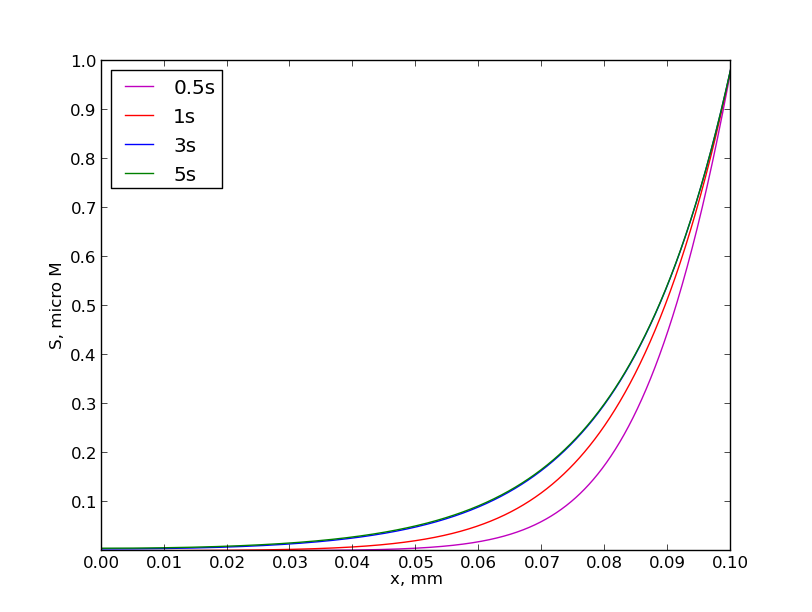
\includegraphics[scale=0.5]{img/S}
    \caption{Substrate}
    \label{img:mlp}
\end{figure}

\begin{figure}[H]
    \centering
    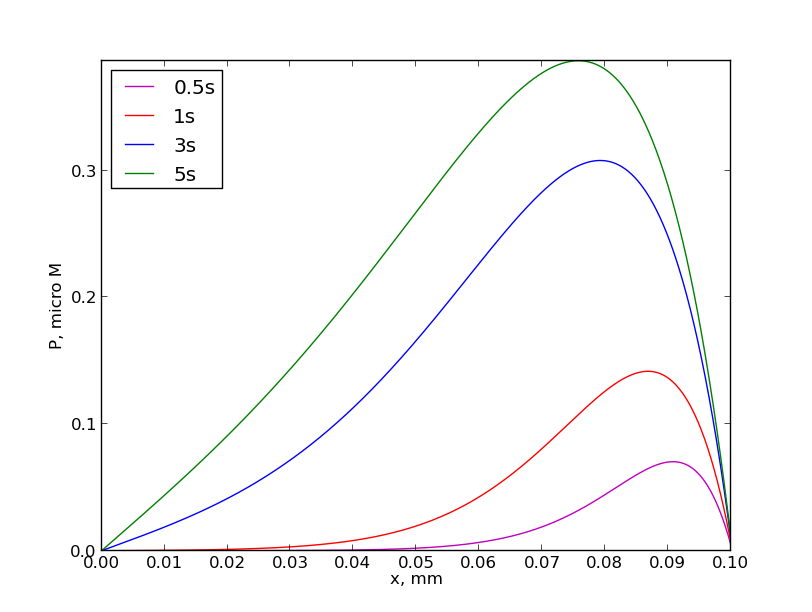
\includegraphics[scale=0.5]{img/P}
    \caption{Product}
    \label{img:mlp}
\end{figure}

\begin{figure}[H]
    \centering
    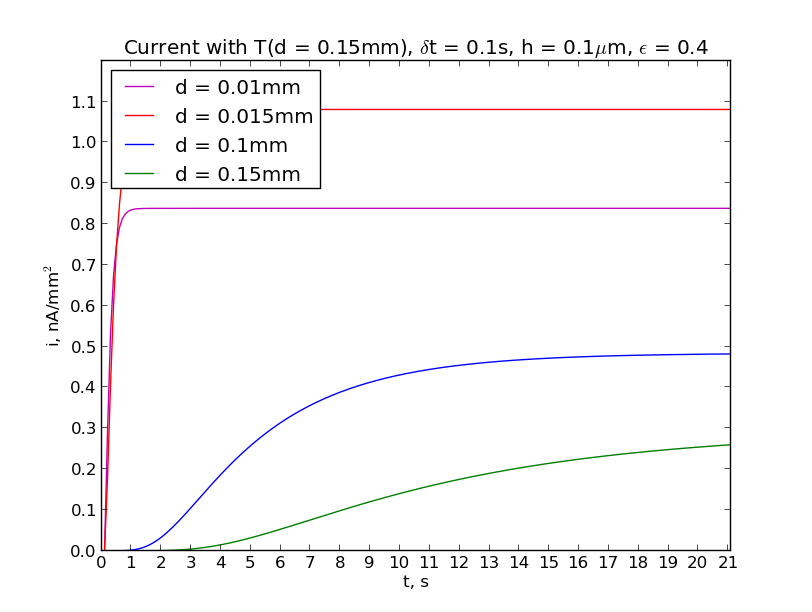
\includegraphics[scale=0.5]{img/i}
    \caption{Current}
    \label{img:mlp}
\end{figure}

%\appendix
%----------------------------------------------------

\bibliography{bibliografija}


%\appendix
%\section{Papildomų eksperimentų rezultatų lentelės}
%\begin{figure}[H]
%    \centering
%    \includegraphics[scale=0.5]{img/MLP}
%    \caption{Paveikslėlio pavyzdys}
%    \label{img:mlp}
%\end{figure}
%
\end{document}
